\chapter{模型}

这一章会详细介绍所涉及模型的架构,包括创新点以及各模型之间的不同之处。在\autoref{sec:tef}里,会对标准的Transformer\cite{vaswani2017attention}与其自注意力机制做简要介绍,然后在\autoref{sec:pf}里会详细叙述Poolingformer 模型与其双层注意力机制。在\autoref{sec:deb}里,会介绍Deberta\cite{he2020deberta}模型的相对位置编码,最后在\autoref{sec:pd}详细阐述将Poolingformer与Deberta两个模型结合的细节。

\section{Transformer模型}
\label{sec:tef}

根据任务是否需要生成文本,Transformer可以只包含Encoder编码器,又或者体现为一个Encoder-Decoder架构,包括编码器与解码器,实现信息的理解并用于文本的生成。无论是编码器还是解码器,Transformer都是由多个结构完全相同的层串联在一起形成的,每一层的输出即作为下一层的输入。当然,编码器与解码器的层有一些不同,但其基本组件都是一致的,包括多头自注意力部件,双层前馈神经网络,层正则化\cite{ba2016layer}与其之后的残差连接,具体可以参考\autoref{fig:trfarch}\cite{tay2020efficient}。

对于长度为$N$的输入序列,首先将其嵌入到高维空间,用长度为$d$的向量来表示一个token,此时序列的形状为 $\mathbb{R}^N \times \mathbb{R}^d$。在输入第一层之前,还要加上一个相同形状的位置编码,使得模型可以识别每个token的位置。这个位置编码可以通过训练得到,也可以是用三角函数构造的彼此正交的向量集合。

\begin{figure}
\centering
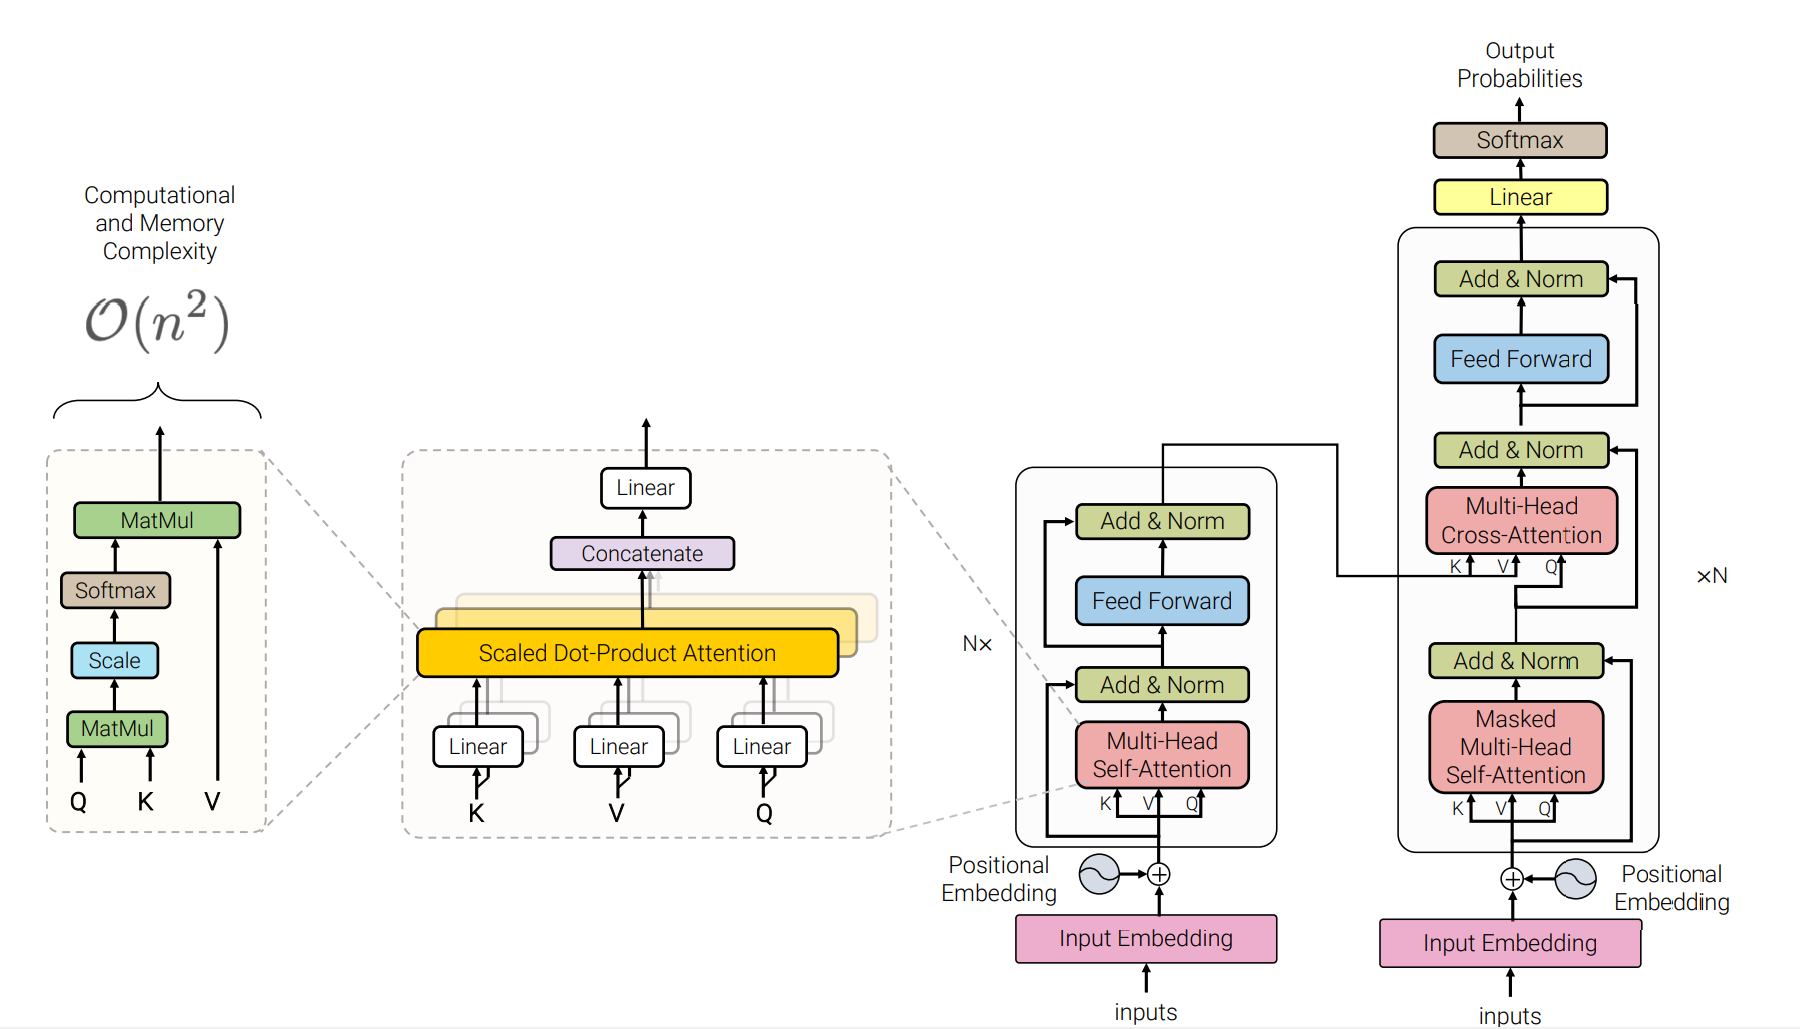
\includegraphics[width=1\textwidth]{trfarch}
\caption{标准Transformer架构}
\label{fig:trfarch}
\end{figure}

以编码器为例,Transformer的每一层中,数据又会先后通过多头自注意力与双层前馈神经网络两大部件,且在经过这两个部件时都要进行正则化与残差连接。每一层的计算可以表示为先执行
\begin{equation}
 	X=\text{LayerNorm}(\text{Self-Attention}(X))+X,
 \label{eq:trfattn}
 \end{equation}
再执行
\begin{equation}
 	X=\text{LayerNorm}(\text{FFN}(X))+X.
 \label{eq:trfffn}
 \end{equation}
解码器的一层比编码器多一个多头交叉注意力组件,将要生成的token与编码器输出的token计算注意力,以融合来自编码器的信息。

\subsection{多头自注意力}

自注意力机制无疑是Transformer模型最重要的部分。对于其中一个头来说,其注意力计算可以表示为:
\begin{equation}
 	\mathbf{A}_h = \text{Softmax}(\alpha \mathbf{Q}_h \mathbf{K}_h^\top)\mathbf{V}_h.
 \label{eq:trfselfattn}
 \end{equation}
其中$\mathbf{Q}_h=\mathbf{W}_q\mathbf{X}$,$\mathbf{K}_h=\mathbf{W}_k\mathbf{X}$,$\mathbf{V}_h=\mathbf{W}_v\mathbf{X}$是经过了三个不同的映射变换的输入序列,分别为query,key,value序列,而$\mathbf{W}_q$,$\mathbf{W}_k$,$\mathbf{W}_v\in \mathbb{R}^{d\times d_h}$则是三个不同的映射矩阵。$\mathbf{X}$是输入序列,而$N_h$表示头的个数,$d_h$表示每个头的嵌入长度。一般来说$d=N_h\times d_h$,所以可以视作每个头都分配了嵌入的一段,进行计算。$\alpha$是正则化因子,一般设置为$\frac{1}{\sqrt{d_h}}$。

用$\mathbf{A}_1,\cdots,\mathbf{A}_{N_h}$表示每个头的输出,则自注意力计算的最后一步是:
\begin{equation}
 	\mathbf{Y} = \mathbf{W}_o [\mathbf{A}_1,\cdots,\mathbf{A}_{N_h}],
 \label{eq:trfselfattnout}
 \end{equation}
$\mathbf{Y}$为自注意力输出,而$\mathbf{W}_o \in \mathbb{R}^{d \times d}$是输出映射矩阵。

通过注意力分数矩阵$\mathbf{A}=\mathbf{Q}\mathbf{K}^\top$的计算,自注意力机制让每个token都能从所有token获得信息。与此同时,这步操作也带来了$\mathcal{O}(n^2)$的时间和空间复杂度,这大大限制了输入序列的长度,以及Transformer在长文本上的应用。

\section{Poolingformer:双层注意力机制}
\label{sec:pf}

由于模型对Transformer的修改仅限于注意力部分,本小节只详细介绍Poolingformer的双层注意力机制。

\subsection{第一层注意力:滑动窗口注意力}

第一层注意力采用了滑动窗口的自注意力机制。在没有全局 token的情况下,每个token之和其前后一定范围内的token,即一个接收窗口内的token计算注意力分数。设$w_1$为窗口长度,则第$i$个token的接收窗口$\mathcal{N}{(i,w_1)}$可以表示为:
\begin{equation}
    \mathcal{N}{(i,w_1)} = \left\{ i - w_1,\cdots, i, \cdots, i + w_1  \right\}.
\label{eq.receptivefield}
\end{equation}
用$\mathbf{K}_{\mathcal{N}{(i,w_1)}}$和$\mathbf{V}_{\mathcal{N}{(i,w_1)}}$来表示$\mathbf{K}$和$\mathbf{V}$的对应列,则第一层注意力的输出$\mathbf{Y}$的第$i$个token$\ y_i$为:
\begin{align}
y_i = \text{Softmax}\left( \alpha q_i \mathbf{K}_{\mathcal{N}{(i,w_1)}}^\top \right) \mathbf{V}_{\mathcal{N}{(i,w_1)}}.
\label{eq:first_att}
\end{align}
可见每个token只和窗口范围$\mathcal{N}{(i,w_1)}$内的token计算了注意力,体现了稀疏自注意力的特点。

有一部分任务需要设置一些特殊的token,而这些token往往需要和整个序列的全部token交换信息。以问答任务为例,在序列中会有作为问题的token,这些token显然是要关注整篇文章,反之整篇文章也要关注这些token。这些token被称为全局 token。
如果输入数据指定了全局 token,那非全局 token的普通token的接受范围除了接收窗口以外,还要包括所有的全局 token。而全局 token要和整个序列全部token计算注意力。以$\mathcal{G} = \{ q_1, \cdots, q_l \}$表示全局 token集合,则第$i$个token的接受窗口$\mathcal{N_G}(i, w_1)$表示为:
\begin{equation}
\mathcal{N_G}(i, w_1) =
\begin{cases}
 \mathcal{N}(i, w_1) \cup \mathcal{G} & i \notin \mathcal{G} \\
 [\![1, \cdots,n]\!] & i \in \mathcal{G}
\end{cases}.
\label{eq:first_win_glb}
\end{equation}
注意力计算修改为:
\begin{align}
y_i = \text{Softmax}\left( \alpha q_i \mathbf{K}_{\mathcal{N_G}{(i,w_1)}}^\top \right) \mathbf{V}_{\mathcal{N_G}{(i,w_1)}}.
\label{eq:first_att_global}
\end{align}

\subsection{第二层注意力:池化}

第二层注意力是一种基于池化(pooling)的注意力机制。对第一层注意力的输出$\mathbf{Y}$进行映射
\begin{align}
\mathbf{\widetilde{Q}}=\mathbf{W}_{\widetilde{q}}\mathbf{Y},\\
\mathbf{\widetilde{K}}=\mathbf{W}_{\widetilde{k}}\mathbf{Y},\\
\mathbf{\widetilde{V}}=\mathbf{W}_{\widetilde{v}}\mathbf{Y}.
\label{eq:second_att_input}
\end{align}
得到变换后的query,key与value序列$\mathbf{\widetilde{Q}},\mathbf{\widetilde{K}},\mathbf{\widetilde{V}}$,$\mathbf{W}_{\widetilde{q}},\mathbf{W}_{\widetilde{k}},\mathbf{W}_{\widetilde{v}}$是不同于第一层注意力的新的映射矩阵。每个token的关注范围仍然是之和其前后一定范围内的token,而窗口长度$w_2$要比第一层的窗口长度$w_1$要大,从而token能够看到更大范围的内容,极端情况下,$w_2$也可以等于序列长度,这样token的接受窗口就都是整个序列了。

在扩大信息接受面的同时,为了达到节省计算资源的目的,Poolingformer会对接受窗口(以第$i$个token为例)$\mathcal{N}(i, w_2)$所对应的序列$\widetilde{\mathbf{{K}}}_{\mathcal{N}(i, w_2)}$与$\widetilde{\mathbf{{K}}}_{\mathcal{N}(i, w_2)}$进行池化操作:
\begin{align}
    \bar{\mathbf{K}}_i &= \text{Pooling}( \widetilde{\mathbf{{K}}}_{\mathcal{N}(i, w_2)}; \kappa, \xi), \\
    \bar{\mathbf{V}}_i &= \text{Pooling}( \widetilde{\mathbf{{V}}}_{\mathcal{N}(i, w_2)}; \kappa, \xi),
\label{eq:pool}
\end{align}
其中$\bar{\mathbf{K}}_i$,$\bar{\mathbf{V}}_i$表示经过池化的key,value序列,$\kappa$,$\xi$表示池化的核大小与步长。在池化操作中,每隔$\xi$个token,就会由相邻的$\kappa$个token计算得到一个token。因此,经过池化后,$\bar{\mathbf{K}}_i$与$\bar{\mathbf{V}}_i$的长度比$\widetilde{\mathbf{{K}}}_{\mathcal{N}(i, w_2)}$,$\widetilde{\mathbf{{V}}}_{\mathcal{N}(i, w_2)}$短了$\kappa$倍,通过池化操作,达到了缩短序列长度,压缩信息的目的,实际的窗口长度只有$\frac{w_2}{\kappa}$,节省了计算资源。

所以第二层注意力输出$\mathbf{Z}$的第$i$个token$\ z_i$为:
\begin{align}
z_i = \text{Softmax}\left( \alpha \widetilde{q}_i \bar{\mathbf{K}}_{i}^\top \right) \bar{\mathbf{V}}_{i}.
\label{eq:second_att}
\end{align}
Poolingformer以残差连接的形式串联了第一层与第二层注意力,经过两层注意力计算后的输出$\mathbf{X}$可以表示为:
\begin{align}
\mathbf{X} = \mathbf{W}_o(\mathbf{Y}+\mathbf{Z}),
\label{eq:second_att_out}
\end{align}
其中$\mathbf{W}_o \in \mathbb{R}^{d \times d}$是输出映射矩阵。

池化,压缩操作的种类很多,本文选择了均值,最大值,卷积三种进行实验对比,并将实验结果记录于()节中。其中,卷积池化采用的是由\cite{wu2019pay}介绍的一种需要训练的轻量级动态卷积池化机制。本实验中,以$(v_1,...,v_\kappa)$作为一个卷积核的token序列片段,卷积结果为:
\begin{align}
\operatorname{LDConv}(v_1,...,v_\kappa)=\sum_{i=1}^{\kappa} \delta_{i} \cdot v_i .
\label{eq:LDConv}
\end{align}
其中$(\delta_1,...,\delta_\kappa)$为动态卷积权重,由片段的中心token$v_{\lceil \frac{1+\kappa}{2} \rceil}$通过一个可训练映射矩阵$\mathbf{W}_p$进行映射得到,即
\begin{align}
    (\delta_1, ..., \delta_\kappa)^T = \text{Softmax}(\mathbf{W}_p v_i).
\end{align}

\subsection{复杂度分析}

在第一层注意力中,如果没有全局 token,每个token只要和接收窗口内的$2w_1$个token计算注意力,所以复杂度为$\mathcal{O}(w_1n)$。若有$g$个全局 token,每个token则多和这$g$个token计算注意力,增加的复杂度为$\mathcal{O}(gn)$。在第二层注意力中,池化后的接收窗口序列长为$\frac{w_2}{\kappa}$,所以其复杂度为$\mathcal{O}(\frac{w_2}{\kappa}n)$。$w_1$,$g$,$w_2$都是可以设置的参数,相对较小且与序列长度无关,所以对整个Poolingformer模型来说,时空复杂度为$\mathcal{O}(n)$。这意味着资源开销只随着序列长度线性增长,解决了Transformer模型$\mathcal{O}(n^2)$复杂度,面对长文本任务时资源开销过大的问题。

%Poolingformer与Deberta的融合模型
\section{Deberta的相对位置编码机制}
\label{sec:deb}

Deberta\cite{he2020deberta}的相对位置编码的核心思想便是表征两个token之间的相对位置关系。在Transformer的自注意力计算中,计算两个token的注意力分数时,只需要进行一次点乘$QK^\top$,query与key都主要携带着token内容相关的信息。而Deberta在计算分数时需要三次点乘;以第$i$与第$j$个token为例,除了两者的内容分数$QK^\top$外,还要将query与key分别与两者相对位置的表征$P_{i\mid j}$与$P_{j\mid i}$进行点乘,再将三者的结果相加作为两个token的注意力分数。可以说,Deberta的注意力分数是由内容-内容,内容-位置,位置-内容三部分组成的。
以$k$表示最大相对位置,则第$i$相对于第$j$个token的位置$\delta(i,j)$表示为:
\begin{equation}
\delta(i,j)=
\begin{cases}
0 & i-j\le -k \\
2k-1 & i-j\ge k \\
i-j+k & -k<i-j<k
\end{cases}.
\label{eq:rel_pos}
\end{equation}
自注意力计算可以表示为:
\begin{align}
\widetilde{A}_{i,j}=\mathbf{Q}^c_i {\mathbf{K}^c_j}^\top + \mathbf{Q}^c_i {\mathbf{K}^r_{\delta(i,j)}}^\top +  \mathbf{K}^c_j {\mathbf{Q}^r_{\delta(j,i)}}^\top,\\
\mathbf{Y}=\text{Softmax}(\alpha\mathbf{\widetilde{A}})\mathbf{V}_c.
\label{eq:deberta_att}
\end{align}
$\mathbf{Q}_c = \mathbf{W}_{q,c}\mathbf{X},\mathbf{K}_c = \mathbf{W}_{k,c}\mathbf{X},\mathbf{V}_c = \mathbf{W}_{v,c}\mathbf{X}$是输入序列映射后得到的query,key,value内容序列,而$\mathbf{W}_{q,c},\mathbf{W}_{k,c},\mathbf{W}_{v,c} \in \mathbb{R}^{d \times d}$为对应内容映射矩阵。而$\mathbf{P} \in \mathbb{R}^{2k \times d}$为相对位置编码的嵌入矩阵,Deberta最多可以表征$2k$种相对位置,$\mathbf{P}$的一行就对应了一种相对位置,而且$\mathbf{P}$是模型的全部层共用的。在每一层里,各自不同的$\mathbf{W}_{q,r},\mathbf{W}_{k,r} \in \mathbb{R}^{d \times d}$位置映射矩阵对$\mathbf{P}$映射后,生成$\mathbf{Q}_r = \mathbf{W}_{q,r}\mathbf{P}$与$\mathbf{K}_r = \mathbf{W}_{k,r}\mathbf{P}$为两个经过映射的相对位置编码矩阵。

因为$\mathbf{A}$中的分数是由三项相加得来,正则化因子也改为了$\frac{1}{\sqrt{3d}}$,这能使训练更加稳定。

由于Transformer的序列长度限制一般为512,Deberta将最大相对位置$k$也设为了512。已经训练好的相对位置编码不能再准确表征距离更远的相对位置,这也为Deberta的模型参数用于处理文本更长的任务带来了不便。

\section{Poolingformer与Deberta的融合模型}
\label{sec:pd}

Deberta的相对位置编码可以更准确地编码token的位置信息。因此,将这种相对位置编码引入Pooingformer,引入在第一层的滑动窗口自注意力中,也可以让模型更好的获得位置信息。

在这个融合模型的第一层注意力中,token只和接受窗口里的token计算注意力分数,这一点和Poolingformer一致。而计算分数时,由内容-内容,内容-位置,位置-内容三部分分数再相加得到,这一点和Deberta是一样的。设$w_1$为窗口长度,窗口$\mathcal{N}{(i,w_1)}$为:
\begin{equation}
    \mathcal{N}{(i,w_1)} = \left\{ i - w_1, ..., i, ..., i + w_1  \right\}.
\label{eq.receptivefield2}
\end{equation}
注意力计算公式为:
\begin{align}
%\widetilde{A}_{i,j}=\mathbf{Q}^c_i {\mathbf{K}^c_\hat{j}}^\top + \mathbf{Q}^c_i {\mathbf{K}^r_{\delta(i,\hat{j})}}^\top +  \mathbf{K}^c_\hat{j} {\mathbf{Q}^r_{\delta(\hat{j},i)}}^\top\\
\widetilde{A}_{i,j}=\mathbf{Q}^c_i {\mathbf{K}^c_j}^\top + \mathbf{Q}^c_i {\mathbf{K}^r_{\delta(i,j)}}^\top +  \mathbf{K}^c_j {\mathbf{Q}^r_{\delta(j,i)}}^\top,\\
\mathbf{Y}=\text{Softmax}(\alpha\mathbf{\widetilde{A}})\mathbf{V}_c.
\label{eq:pooldeberta_att}
\end{align}
因为只和接收窗口里的token计算注意力,所以$j \in  \mathcal{N}{(i,w_1)}$。

值得注意的是,在没有全局 token时,在滑动窗口自注意力的限制下,最远的相对位置的距离绝对值便是窗口长度$w_1$。而相对位置编码$\mathbf{P}$只能表征最长$k$的相对位置,所以必然有
\begin{equation}
    w_1\le k,
\label{eq.limit1}
\end{equation}
不然就会出现相对位置编码不够,或者说越界的情况。幸运的是,消融实验得到的结论是最优$w_1=128$,这也是主实验所使用的设置,满足小于$k=512$的要求,当然这也是Poolingformer能够高效利用距离token最近的这些最有效的信息的证明。

\subsection{全局 token与相对位置编码}

在存在全局 token 的情况下,如果不加以特殊处理,相对位置编码就一定会越界。因为全局 token 要和整个序列进行注意力计算,而且全局 token一般置于整个序列的起始位置,所以最远的相对位置的距离绝对值为序列长度$N$。在长文本的情况下,$N$可以为4096乃至16384,远远大于$k=512$。

为了解决这个问题,在计算全局 token与其他token的注意力时,必须有额外的相对位置编码以供使用。因此,融合模型设置了额外的全局相对位置编码表征$\mathbf{P}_g \in \mathbb{R}^{2k_g} \times d$,$k_g$为额外设置的表征对的数量,每一对表征包括相对位置为正、负的情况各一。当计算全局 token与其他token的注意力时,注意力分数A的计算公式改为:
\begin{align}
\widetilde{A}_{i,j}=\mathbf{Q}^c_i {\mathbf{K}^c_j}^\top + \mathbf{Q}^c_i {\mathbf{K}^{r,g}_{\mathcal{F}(\delta(i,j))}}^\top +  \mathbf{K}^c_j {\mathbf{Q}^{r,g}_{\mathcal{F}(\delta(i,j))}}^\top ,
\label{eq:pooldeberta_att_glb}
\end{align}
其中$\mathbf{Q}_{r,g},\mathbf{K}_{r,g}$为经过映射的全局相对位置编码矩阵,而$\mathbf{W}_{q,r,g},\mathbf{W}_{k,r,g} \in \mathbb{R}^{d \times d}$仍然为每层不同的位置映射矩阵。$\mathcal{F}$为从相对位置$\delta(i,j)$到全局相对位置编码表征序号的映射,由相对位置决定使用哪个全局相对位置编码表征,即$\mathbf{P}_g$的哪一列。$\mathcal{G}$为全局 token集。
为了节省显存,使$\mathbf{P}_g$不至于太大,$k_g$设置为远小于$N$,即将$k_g$个表征均匀连续地分配给$N$个相对位置编码是比较合理的方案。几个相邻的相对位置能共用一个编码,节省了空间且不会对模型对相对位置的感知能力造成太多损害,在距离已经很远的情况下,准确的距离信息也不是必须的,模糊的信息,知道大概有多远就足够了。

融合模型的第二层注意力与Poolingformer相同。





